\documentclass[12pt,letterpaper]{article}
\usepackage[utf8]{inputenc}
\usepackage{amsmath}
\usepackage{amsfonts}
\usepackage{amssymb}
\usepackage{amsthm}
\usepackage{graphicx}

\usepackage{tabularx}
\usepackage[left=2cm,right=2cm,top=2cm,bottom=2cm]{geometry}
\usepackage{fancyhdr}
\usepackage{multicol}
\usepackage{multirow,array}
\usepackage{newtxtext,newtxmath}
\usepackage{relsize}
\usepackage{lastpage}
\usepackage{enumitem}
\usepackage{adjustbox}
\newcolumntype{Y}{>{\centering\arraybackslash}X}
\pagestyle{fancy}
\fancyhf{}
\lhead{\textsc{BHCC Mat-181}}
\chead{\textsc{Answers}}
\rhead{\textsc{Exercises 3.1-3.8}}
\rfoot{Page \thepage ~of \pageref{LastPage}}
\setenumerate[1]{label={\bf 3.\theenumi: }}
\setenumerate[2]{label={\bf (\theenumii): }}

\begin{document}

\begin{enumerate}
\setcounter{enumi}{0}
\item \begin{enumerate}
\item Below is a detailed sketch.
\begin{center}
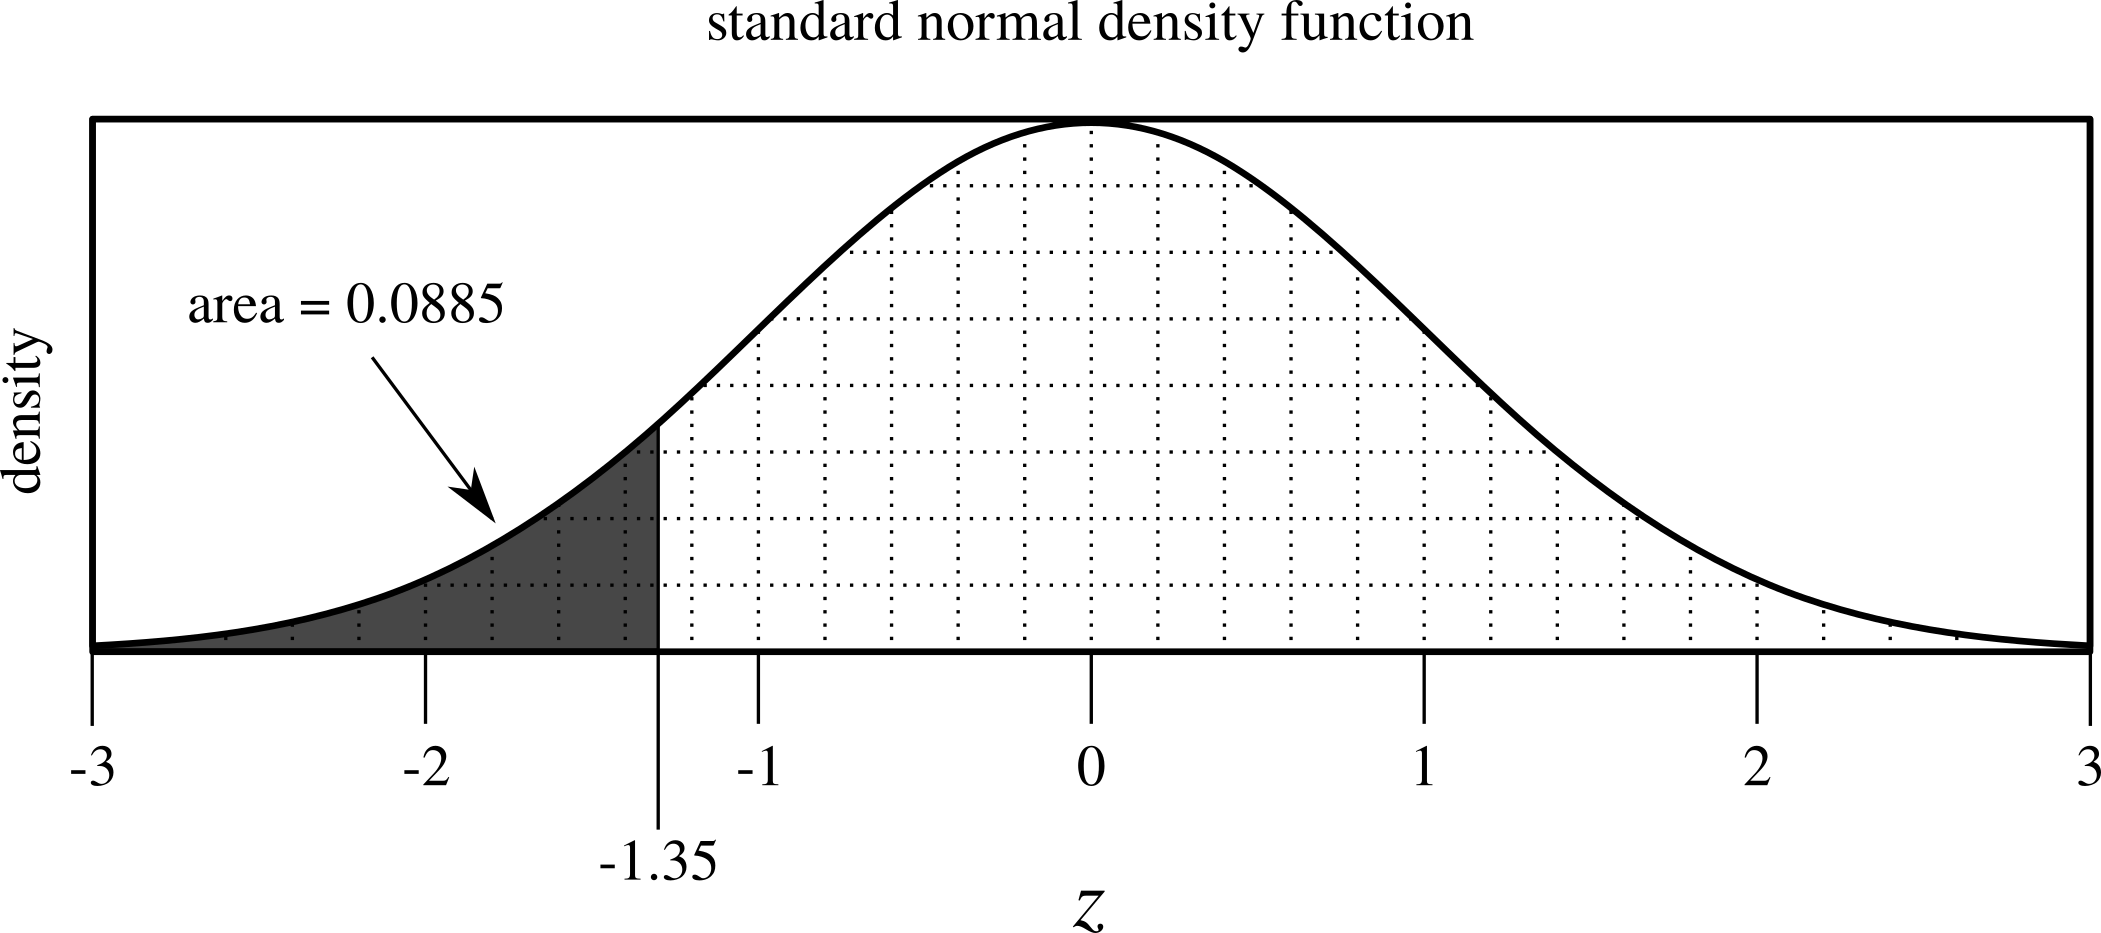
\includegraphics[scale=0.8]{figures/hw3p1a.png}
\end{center}
We are finding a {\bf left} area. This is the easiest. We can use the standard normal table directly.
$$P(Z<-1.35)~~ =~~ \fbox{0.0885} $$
\vfill
\item Below is a detailed sketch.
\begin{center}
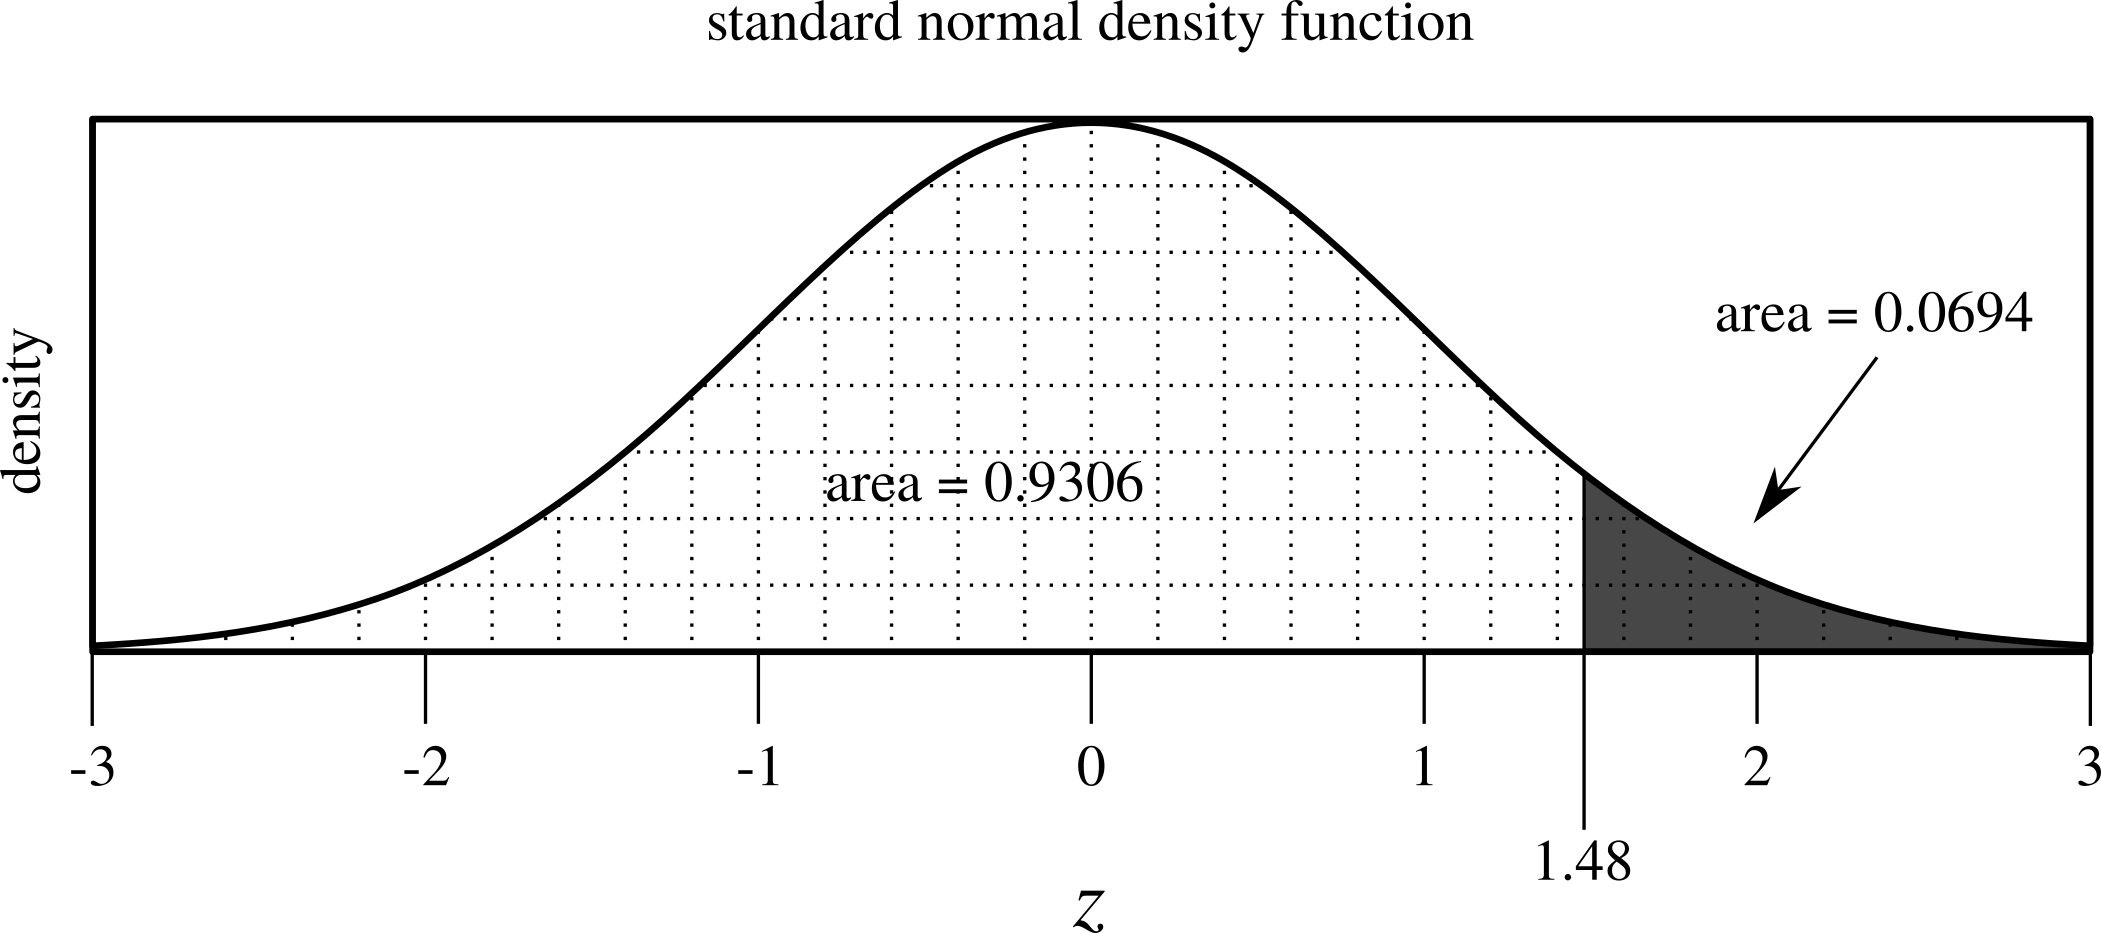
\includegraphics[scale=0.8]{figures/hw3p1b.png}
\end{center}
We are finding a {\bf right} area. We can find the complementary left area from the table.
$$P(Z<1.48)~~ =~~ 0.9306 $$
Then, we can calculate the desired probability.
$$P(Z>1.48)~~ =~~ 1-0.9306 ~~=~~ \fbox{0.0694} $$
\vfill
\newpage
\item Below is a sketch of the area we wish to determine (along with the answer).
\begin{center}
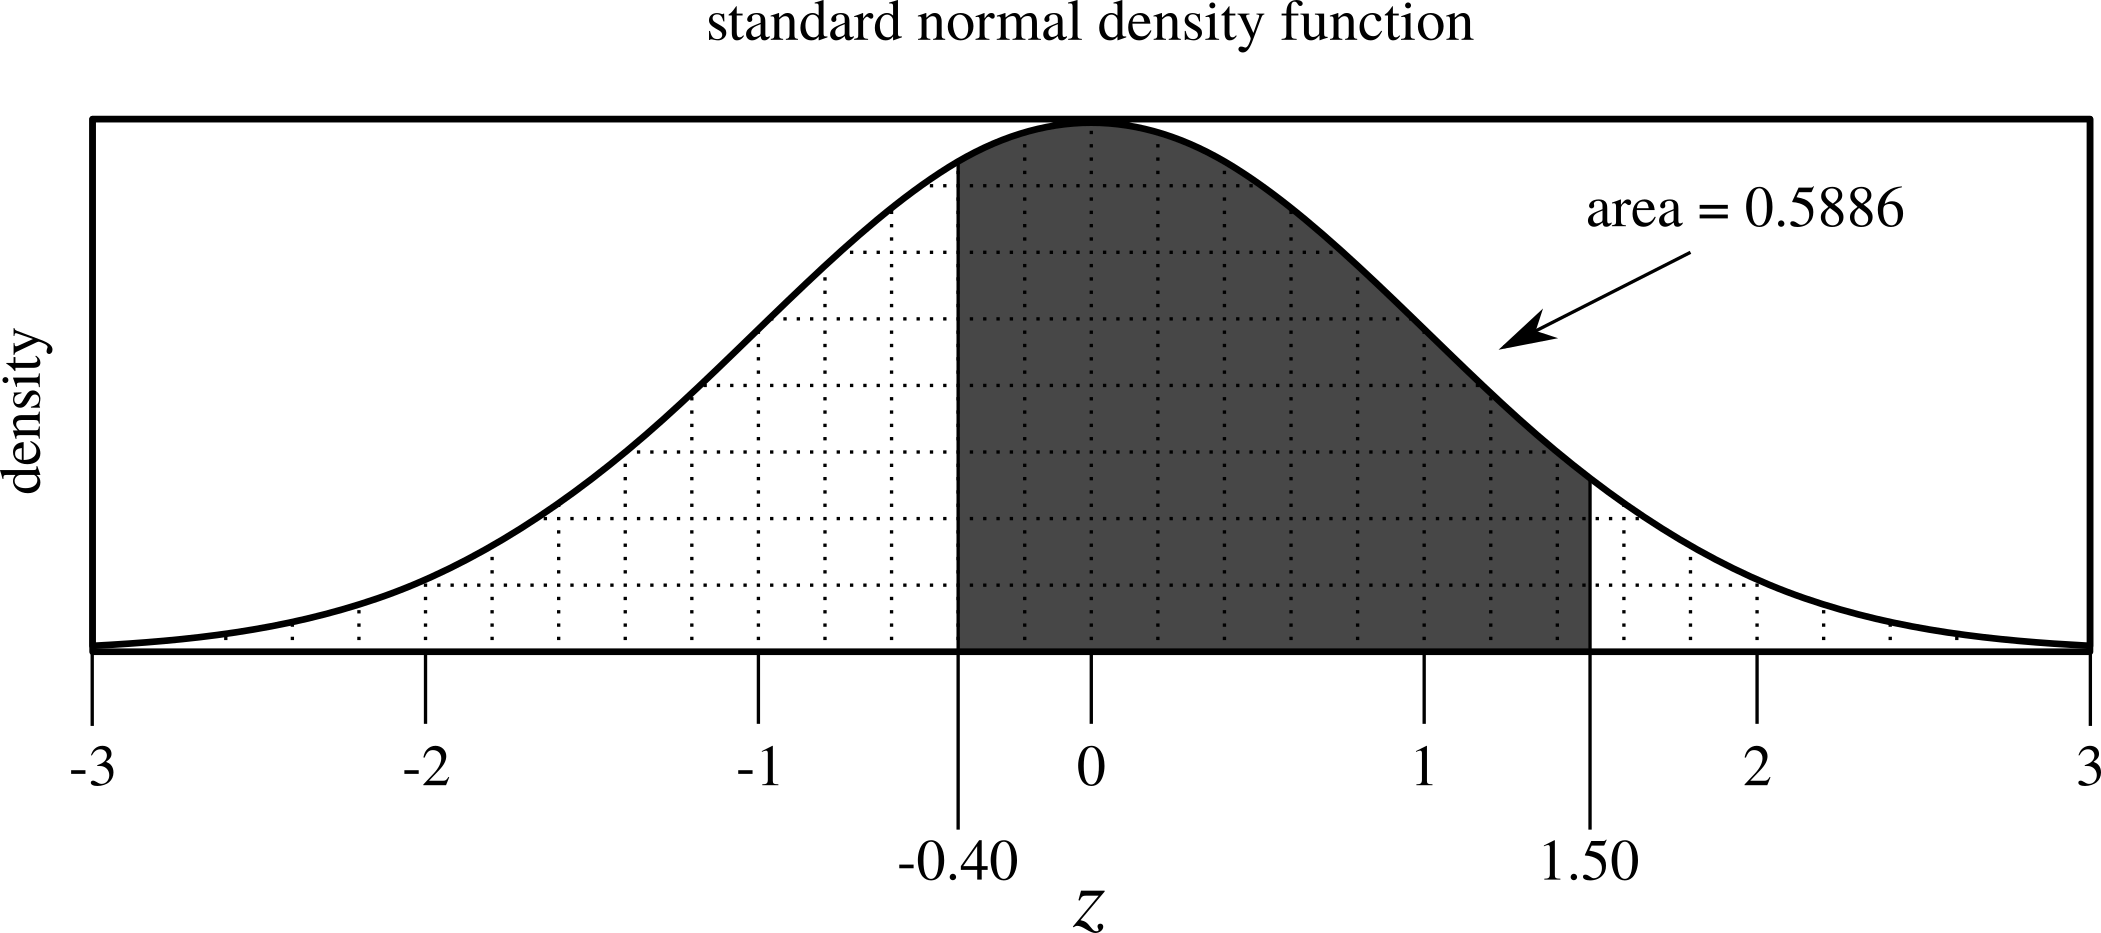
\includegraphics[scale=0.8]{figures/hw3p1c.png}
\end{center}
I'll call this doubly bounded area a {\bf sectional} area. In order to use the table, we will need to subtract two left areas.
$$P(Z<1.5)~~ =~~ 0.9332 $$
$$P(Z<-0.4)~~ =~~ 0.3446 $$
$$P(-0.4 < Z < 1.5)~~ =~~ 0.9332-0.3446 ~~=~~ \fbox{0.5886} $$
\vfill
\item Below is a sketch of the (symmetric) {\bf two-tailed} area we wish to determine.
\begin{center}
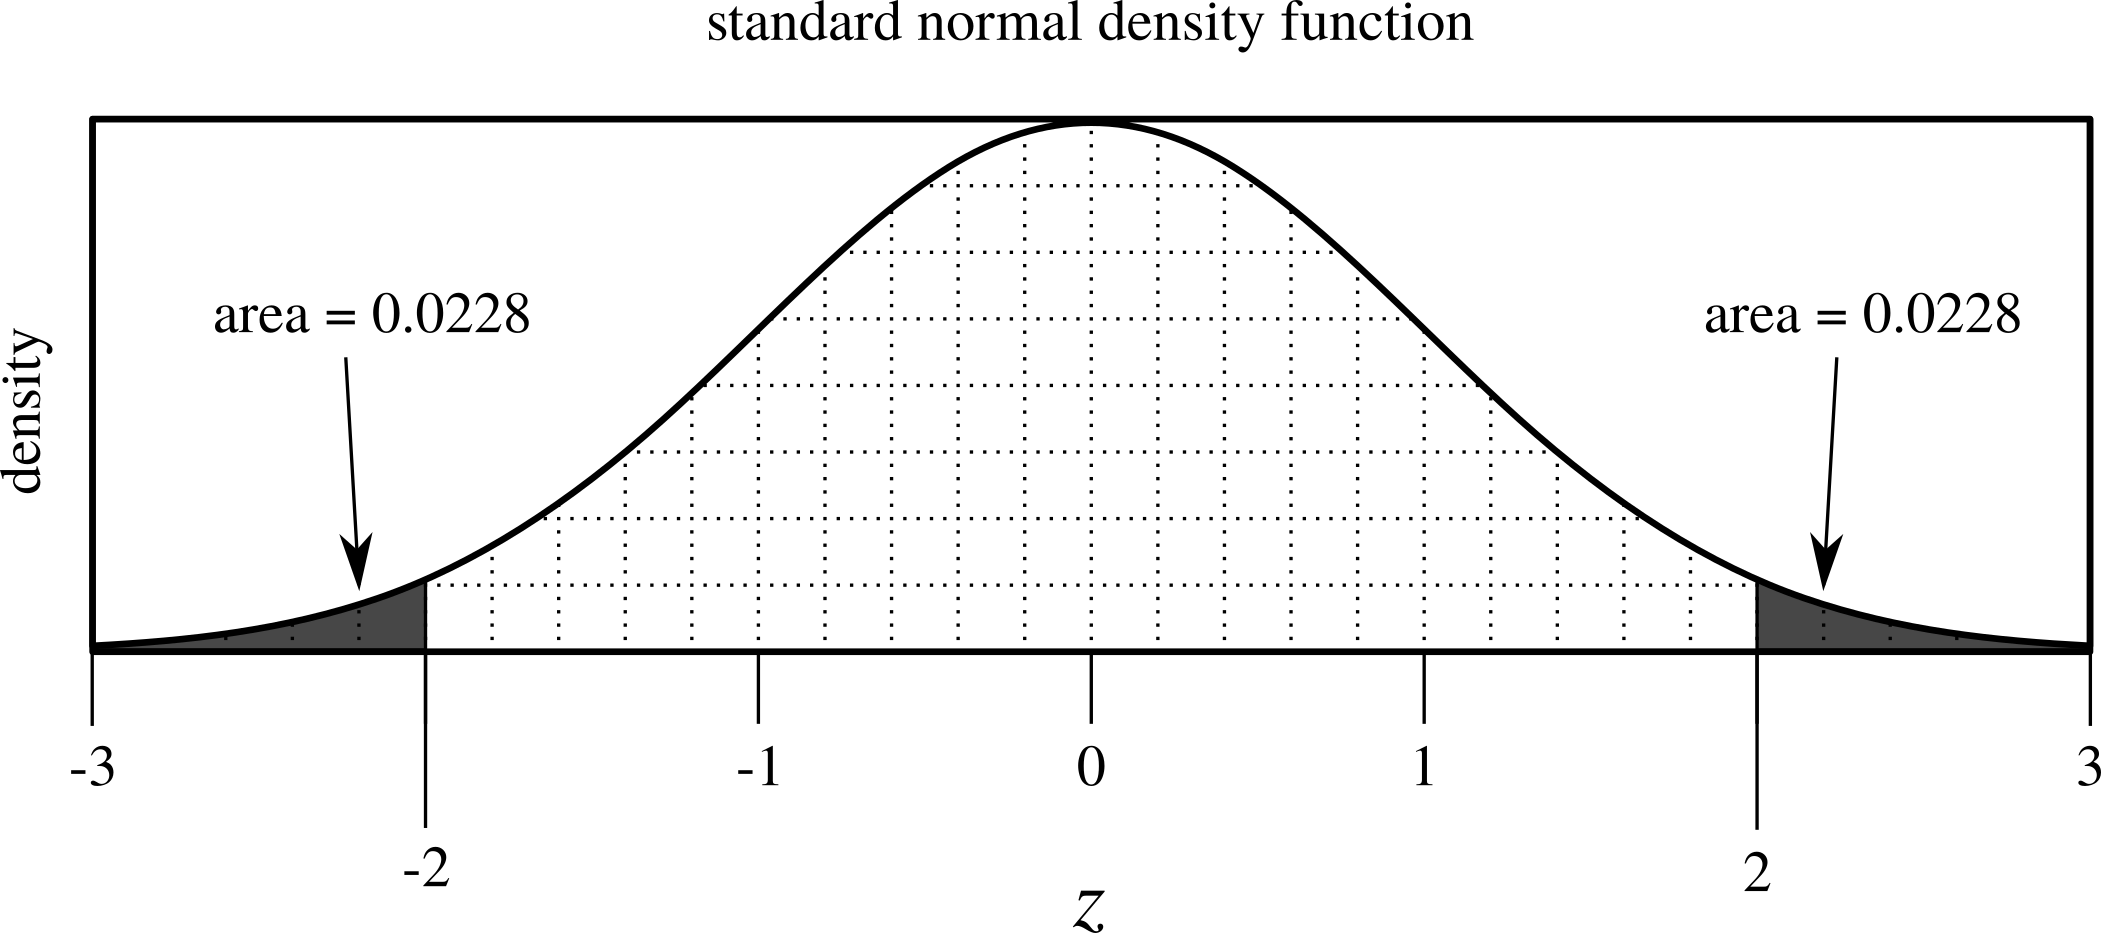
\includegraphics[scale=0.8]{figures/hw3p1d.png}
\end{center}
There are a few ways to find this two-tailed area. Either way we need the left area.
$$P(Z<-2) = 0.0228 $$
In this case, we can use symmetry to find the two-tailed area.
$$P(|Z|>2) ~~=~~ 0.0228+0.0228 ~~=~~ \fbox{0.0456} $$
\vfill
\end{enumerate}

\newpage
\item \begin{enumerate}
\item Below is a detailed sketch.
\begin{center}
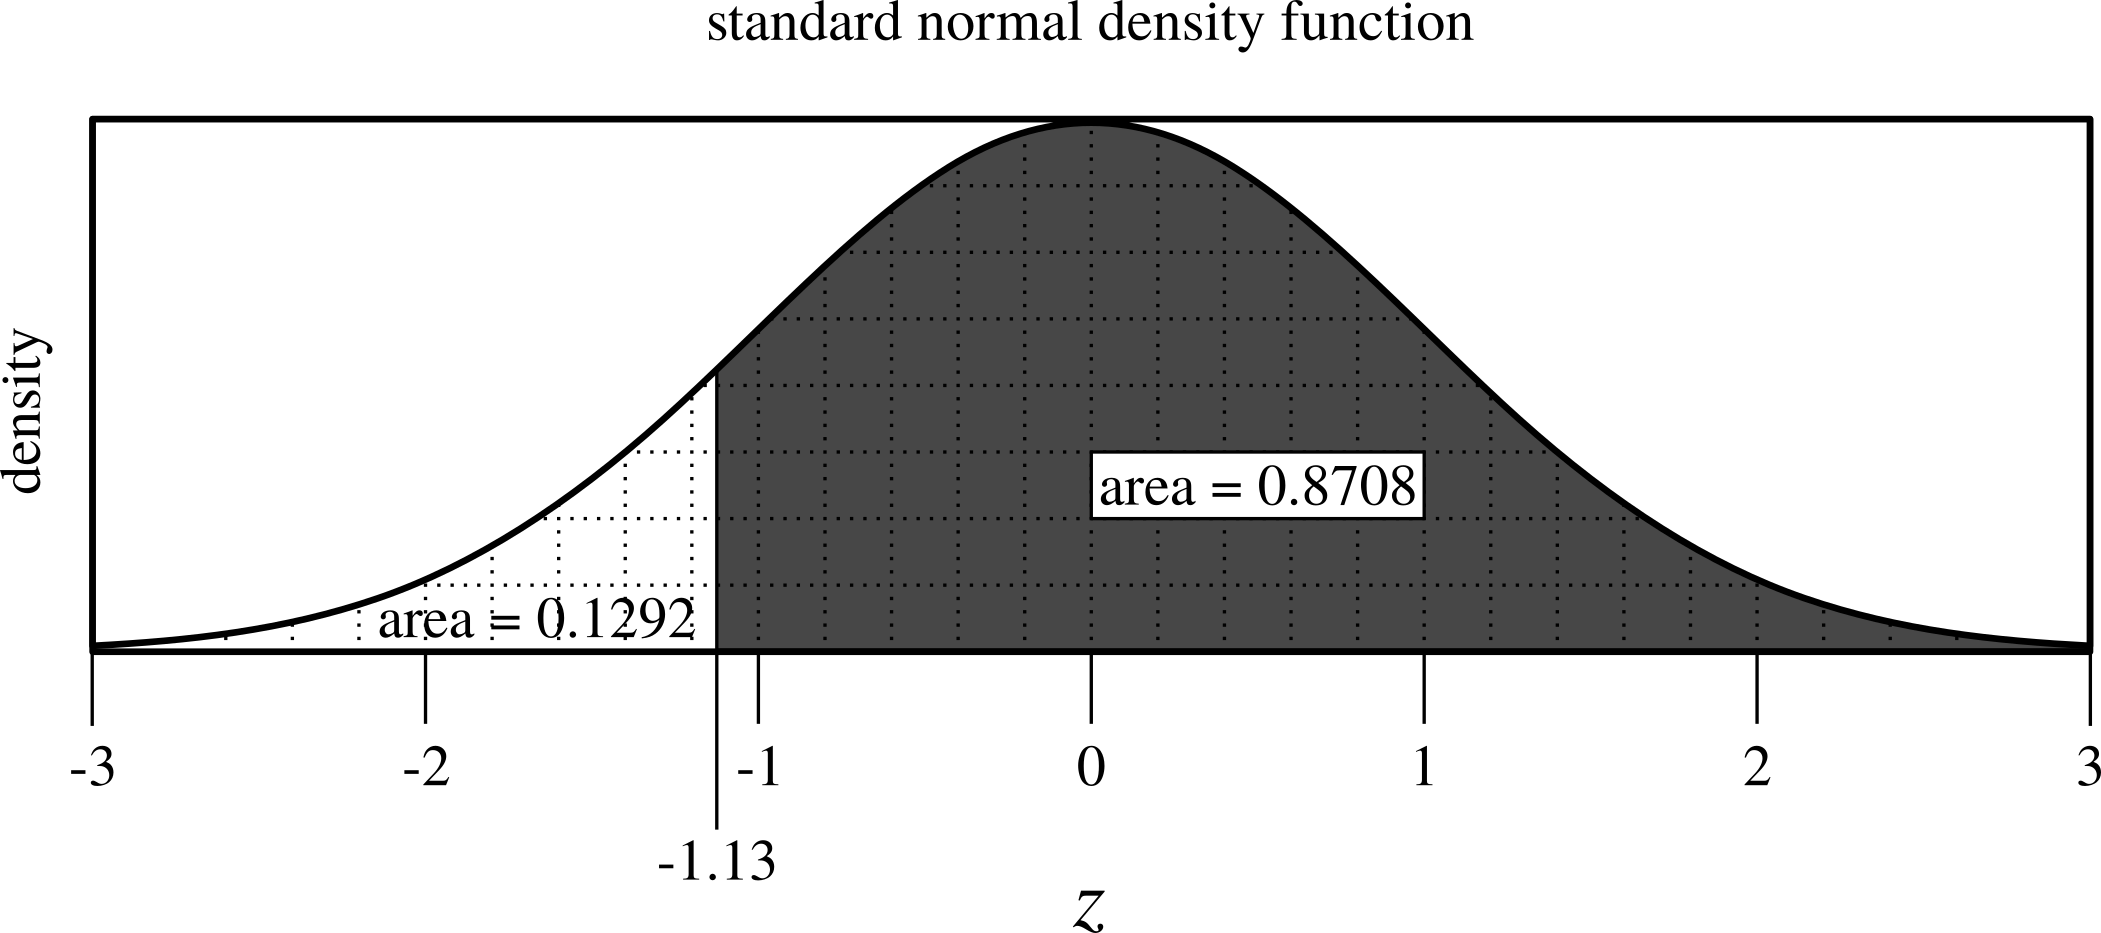
\includegraphics[scale=0.8]{figures/hw3p2a.png}
\end{center}
We are finding a {\bf right} area.
$$P(Z<-1.13)~~ =~~ 0.1292 $$
$$P(Z>-1.13)~~ =~~ 1-0.1292 ~~=~~ \fbox{0.8708} $$
\vfill
\item Below is a detailed sketch.
\begin{center}
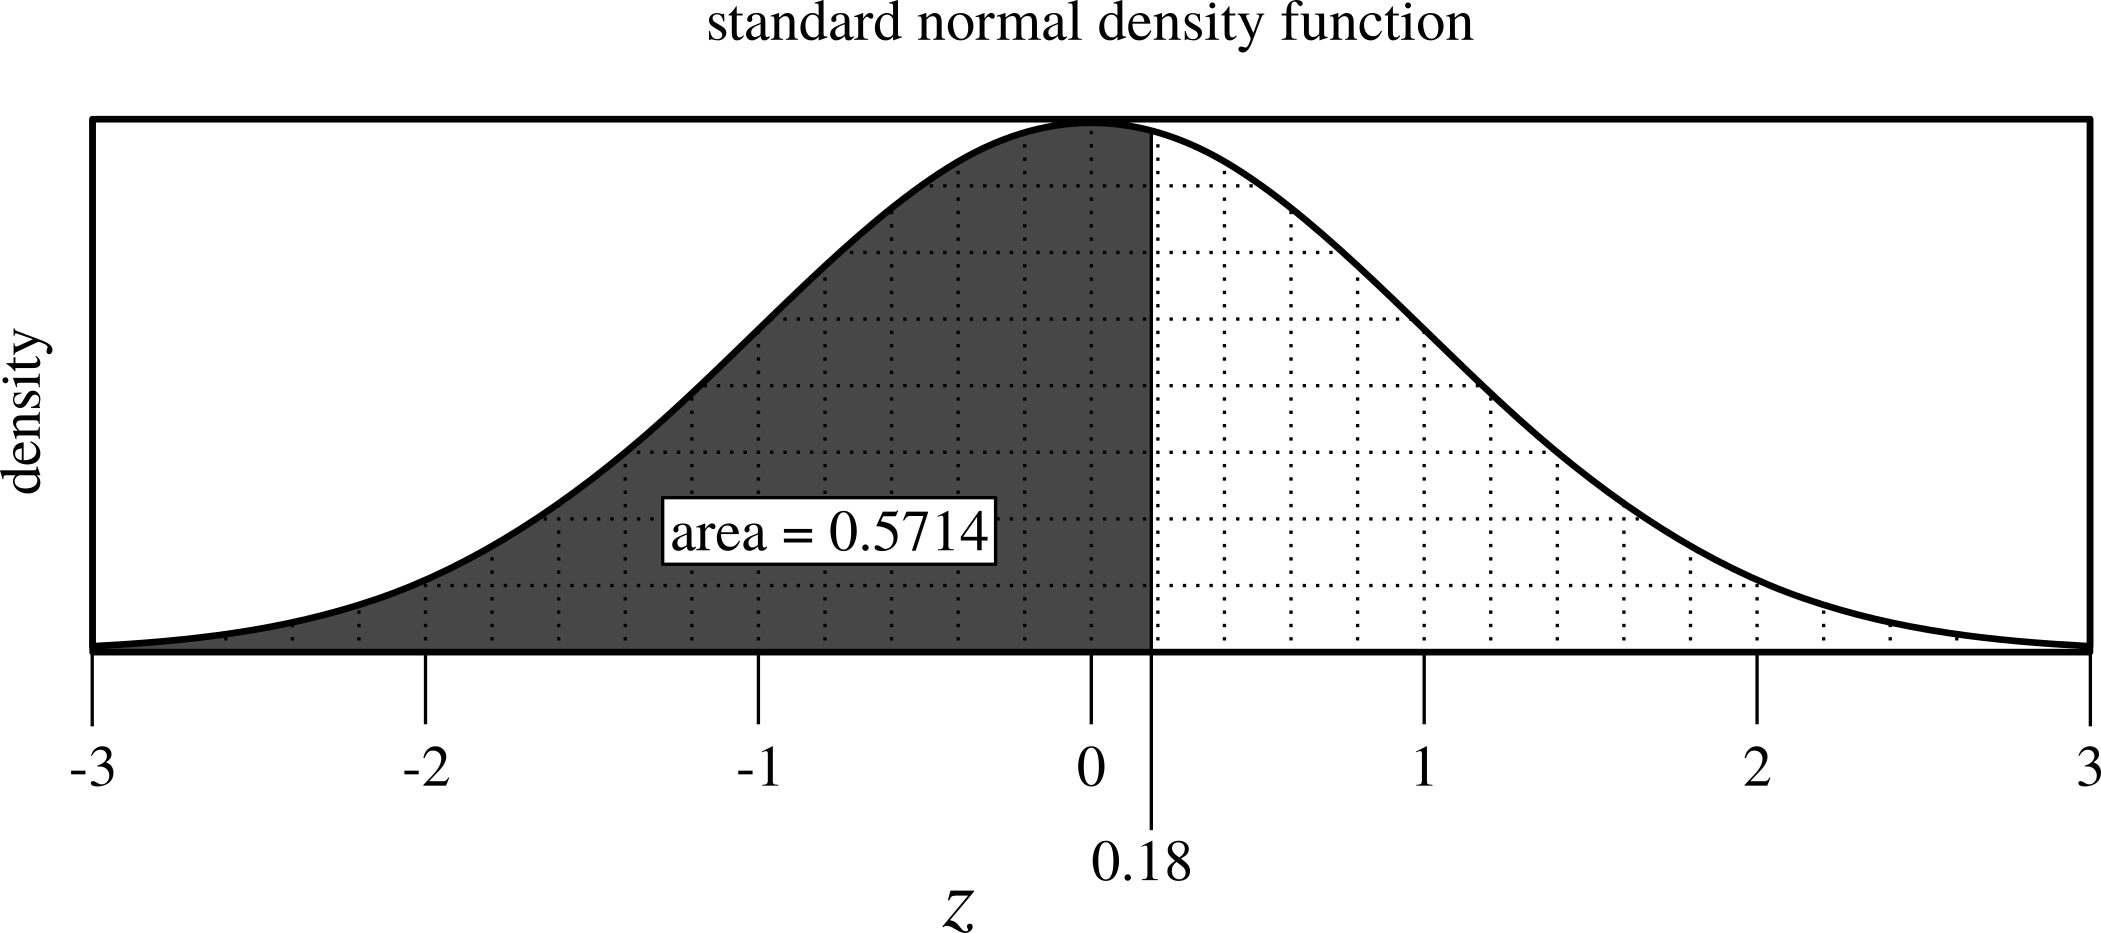
\includegraphics[scale=0.8]{figures/hw3p2b.png}
\end{center}
We are finding a {\bf left} area.
$$P(Z< 0.18)~~ =~~ \fbox{0.5714} $$
\vfill

\newpage

\item The area above $z=8$ is so tiny that we can call it 0. If you have a more advanced way to look this up than the table, you might find a more precise answer: 
$$P(X > 8) = 0.000000000000000622 ~~=~~ 6.22 \times 10^{-16}$$
However, from the table we can conclude the area is {\bf less than {0.0002}}.
\vfill

\item Below is a sketch of the (symmetric) {\bf central} area we wish to determine.
\begin{center}
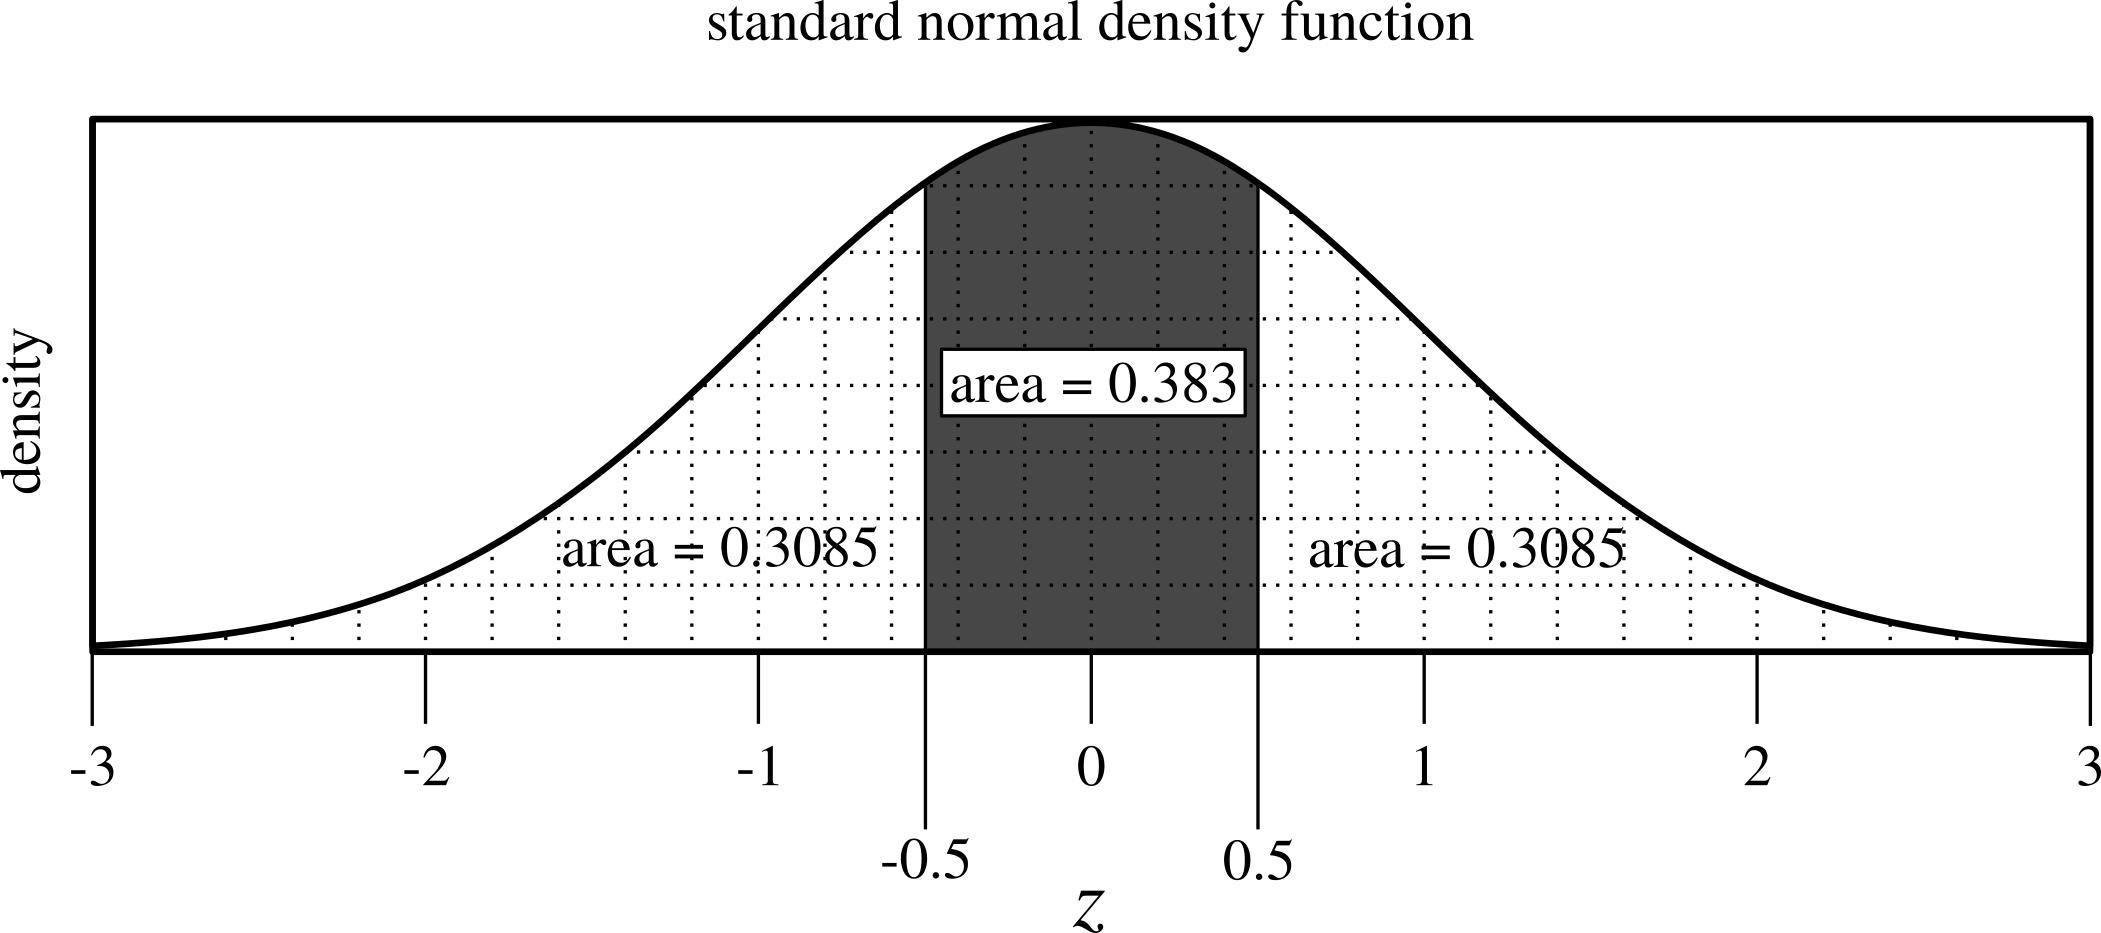
\includegraphics[scale=0.8]{figures/hw3p2d.png}
\end{center}
There are a few ways to find this central area. I like to find the left area of the left boundary.
$$P(Z<-0.5) = 0.3085 $$
We can use symmetry to find the central area.
$$P(|Z|<0.5) ~~=~~ 1-0.3085-0.3085 ~~=~~ \fbox{0.383} $$
I will point out that if you do this with precise software, you will get 0.3829 instead...
\vfill
\end{enumerate}

\newpage
\newcommand{\N}[2]{\mathcal{N}\Big(#1,~ #2\Big)}

\item \begin{enumerate}
\item Let random variable $V$ represent the Verbal Reasoning score of a random person. Let random variable $Q$ represent the  Quantitative Reasoning score of a random person.
$$V \sim \N{151}{7}$$ 
$$Q \sim \N{153}{7.67}$$ 
\newcommand{\zv}{Z_{\textsc{v}, \text{ Sophia}}}
\newcommand{\zq}{Z_{\textsc{q}, \text{ Sophia}}}
\item We calculate the $z$-scores.
$$\zv ~=~ \cfrac{160-151}{7} ~=~ 1.29$$
$$\zq ~=~ \cfrac{157-153}{7.67} ~=~ 0.5215$$
\item Sophia's score on Verbal was 1.29 standard deviations above the mean. Sophia's score on Quantitative was 0.52 standard deviations above the mean.
\item Relative to other people, Sophia did better on Verbal Reasoning.
\item To find her percentile, we need to use the $Z$ table. At this point I want to introduce a new syntax.
$$\Phi(k) \equiv P(Z<k) $$
Basically, $\Phi(z)$ means use the standard normal table with the given value of $z$.
$$\Phi(1.29) = 0.90 $$
$$\Phi(0.52) = 0.70 $$
Sophia was 90th percentile in Verbal and 70th percentile in Quantitative.
\item 10\% did better than Sophia on Verbal. 30\% did better than Sophia on Quantitative.
\item We are more interested in which test Sophia does unusually well on compared to others, not just the raw score.\\
Analogy: just because a specific watermelon might be bigger than a specific orange does not mean the watermelon is more unusually large. 
\item The answer to (b) is the same. I guess (c) is still valid too. The other answers would need to change because they used a normal assumption.
\end{enumerate}

\newpage

\item \begin{enumerate}
\item Let random variable $M$ represent the finishing time of a random man from ages 30 to 34. Let random variable $W$ represent the finishing time of a random woman from ages 25 to 29.
$$M \sim \N{4313}{583}$$ 
$$W \sim \N{5261}{807}$$ 
\newcommand{\zl}{Z_{\text{Leo}}}
\newcommand{\zm}{Z_{\text{Mary}}}
\item We calculate the standard scores. Let $\zl$ represent Leo's standard score. Let $\zm$ represent Mary's standard score.
$$\zl ~=~ \cfrac{4948-4313}{583} ~=~ 1.09$$
$$\zm ~=~ \cfrac{5513-5261}{807} ~=~ 0.31$$
Leo finished 1.09 standard deviations later than average. Mary finished 0.31 standard deviation later than average.
\item Mary ranked better in her group because her standard score is lower.
\item We first find the percent who were faster than Leo by using the table.
$$\Phi(1.09) = 0.8621 $$
Then, we can determine the percent who were slower (had longer times).
$$1-0.8621 = \fbox{0.1379} $$
\item We first find the percent who were faster than Mary by using the table.
$$\Phi(0.31) = 0.6217 $$
Then, we can determine the percent who were slower (had longer times).
$$1-0.6217 = \fbox{0.3783} $$
\item Our answers to (b) and (c) would still be valid. The others need reconsideration as they assumed a normal distribution.
\end{enumerate}

\newpage
\item \begin{enumerate}
\item We now need to use the standard normal table {\bf backwards}. We scan for a percentile nearest 0.8, then determine the value of $Z$ associated with that percentile.
$$\Phi(0.84) = 0.8 $$
I want to introduce another notation, for using the standard normal table in reverse.
$$\Phi(z) = a  ~~\iff ~~ \Phi^{-1}(a) = z $$
Thus, I could write:
$$Z = \Phi^{-1}(0.8) = 0.84 $$
Now, we convert this $Z$ score into a Quantitative Reasoning score.
\begin{align*}
Q &= Z\sigma + \mu \\
  &= (0.84)(7.67) + 153\\
  &= \fbox{159.4}
\end{align*}
\item We find the $Z$ score from the percentile, which is 30th percentile (worse than 70\%).
$$Z = \Phi^{-1}(0.3) = -0.52$$
We calculate the Verbal Reasoning score.
\begin{align*}
V &= Z\sigma + \mu \\
  &= (-0.52)(7) + 151\\
  &= \fbox{147.4}
\end{align*}
\end{enumerate}

\item \begin{enumerate}
\item We find $Z$.
$$Z = \Phi^{-1}(0.05) = -1.64 $$
We find the cutoff time for 5th percentile in Men's.
\begin{align*}
M_\text{5\%} &= Z\sigma + \mu \\
             &= (-1.64)(583) + 4313\\
             &\approx \fbox{3357 \text{ seconds}}
\end{align*}
\item We find $Z$. Remember, this is 90th percentile.
$$Z = \Phi^{-1}(0.90) = 1.28 $$
We find the cutoff time for 90th percentile in Women's.
\begin{align*}
W_\text{90\%} &= Z\sigma + \mu \\
             &= (1.28)(807) + 5261\\
             &\approx \fbox{6294 \text{ seconds}}
\end{align*}
\end{enumerate}

\newpage

\item \begin{enumerate}
\item Let random variable $T$ follow the temperature distribution. We wish to evaluate $P(T\ge 83)$. We first find $Z$.
$$Z = \frac{83-77}{5} = 1.2$$
We use the table (and a sketch).
\begin{align*}
P(T\ge 83) &= P(Z\ge 1.2) \\
             &= 1 - \Phi(1.2)\\
             &= 1 - 0.8849\\
             &= \fbox{0.1151}
\end{align*}
\item We are told to find $x$ such that $P(T \le x) = 0.10$. In other words we are looking for the cutoff of the 10th percentile. We first find the $z$ score.
$$z = \Phi^{-1}(0.1) = -1.28$$
We convert this $z$ into $x$.
\begin{align*}
x &= z\sigma + \mu \\
  &= (-1.28)(5) + 77\\
   &= \fbox{70.6}
\end{align*}
The coldest 10\% of days are below 70.6$^\circ$F.
\end{enumerate}
\newpage
\item \begin{enumerate}
\item Let random variable $R\sim \N{0.147}{0.33}$ represent the annual return. We wish to evaluate $P(R < 0)$.
We calculate the $z$ score.
\begin{align*}
z &= \frac{x-\mu}{\sigma} \\\\
  &= \frac{0-14.7}{33}\\\\
  &= -0.45
\end{align*}
We calculate a left area.
\begin{align*}
P(R < 0) &= P(Z < -0.45) \\
             &= \Phi(-0.45)\\
             &= \fbox{0.3264}
\end{align*}
\item We want to find $x$ such that $P(R>x) = 0.15$. We find $z$ by using the standard normal table in reverse. Also, we are looking for the 85th percentile.
\begin{align*}
z &= \Phi^{-1}(0.85) \\
  &= 1.04
\end{align*}
We convert $z$ into $x$.
\begin{align*}
x &= z\sigma + \mu \\
  &= (1.04)(33) + 14.7\\
   &= \fbox{49.02}
\end{align*}
So, the cutoff is a return of 49 percent. Only in 15\% of years is the return higher than 49\%.
\end{enumerate}

\end{enumerate}
\end{document}